\section{Results}
\label{sec:results}
\subsection{Study population and outcome distribution}
The Kineret clinical study included 48,354 admissions among 29,577 adults with diabetes or inpatient hyperglycemia at six general hospitals \citep{oded2027kineret-jbi}. In this source cohort, 35.3\% of admissions had a documented diabetes diagnosis, 74.7\% met the recurrent-hyperglycemia criterion, and 60.2\% met the extreme-glucose criterion. The criteria overlapped, and patients could qualify on glucose readings alone.

For prediction at day four, both the raw and abstracted histories had to extend beyond the cutoff, allowing time for repeated guideline assessments. This subset comprised 20,994 training, 4,427 validation, and 4,508 test admissions. The test admissions came from 3,193 people. The eligibility percentages above describe the full clinical cohort. Among the day-four test admissions, the frequency of subsequent outcomes ranged from 31.65\% for hyperglycemia to 0.73\% for infection (Table~\ref{tab:outcomes}).

Figure~\ref{fig:support} shows how often the ten candidate complications occurred in the original training set after each observation cutoff from day one to day thirteen. At day four, ketoacidosis and hyperosmolality each fell below the 1\% prevalence threshold. We kept the other eight outcomes throughout the evaluation. Table~\ref{tab:outcomes} gives their frequencies in the date-filtered test set.
\begin{figure}[htbp]
\centering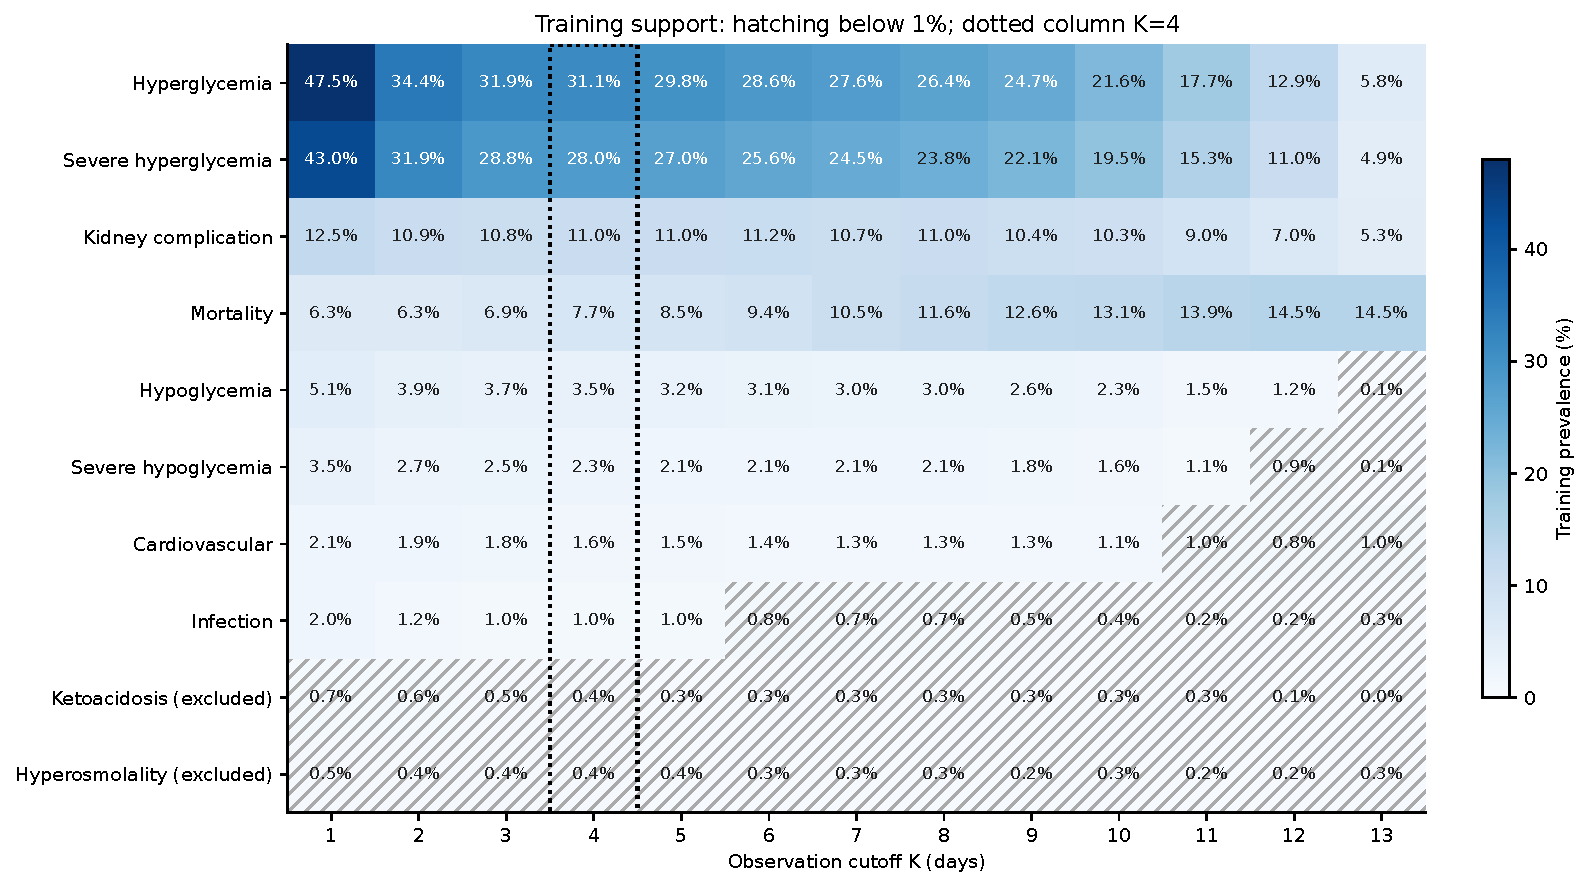
\includegraphics[width=\textwidth]{updated_support_heatmap}
\caption{Prevalence of the ten candidate complications in the original training set. Color indicates the proportion of admissions with an event after cutoff $K$ and through day 14, $(K,14]$. Hatching marks prevalence below 1\%. The dotted outline identifies the cutoff used for outcome selection ($K=4$), and \emph{no head} identifies the excluded outcomes.}
\label{fig:support}
\end{figure}

\subsection{Overall predictive performance and baseline comparisons}
At day four, both comparisons favored clinical intervals (Table~\ref{tab:ladder}). Weighted AUPRC was 0.527 for KB, 0.475 for ss-STraTS, and 0.467 for the SAX interval encoder. The paired gains for KB were 0.053 over ss-STraTS (95\% CI 0.036--0.070) and 0.060 over SAX (0.046--0.076), with $q=0.0012$ for both comparisons. Thus KB improved discrimination even against a model with the same interval encoder. Weighted AUROC also favored KB, and the AUPRC advantage persisted when all outcomes received equal weight.

\begin{table}[htbp]
\centering\small
\caption{Predictive discrimination and length-of-stay error at the four-day observation cutoff.}
\label{tab:ladder}
\resizebox{\textwidth}{!}{\begin{tabular}{lrrrrr}
\toprule
Model & Parameters & Weighted AUPRC & Weighted AUROC & Macro AUPRC & LoS MAE (h) \\
\midrule
Logistic Regression & 25,687 & 0.453 [0.434, 0.475] & 0.751 [0.740, 0.763] & 0.369 & 47.56 \\
Logistic Regression + QA & 26,129 & 0.450 [0.432, 0.472] & 0.751 [0.740, 0.762] & 0.366 & 47.53 \\
\midrule
ss-STraTS & 91,441 & 0.475 [0.456, 0.495] & 0.770 [0.760, 0.781] & 0.370 & 46.27 \\
ss-STraTS + QA & 94,769 & 0.473 [0.456, 0.494] & 0.770 [0.760, 0.781] & 0.360 & 47.48 \\
\midrule
INTERVenE SAX & -- & 0.467 [0.450, 0.488] & 0.762 [0.751, 0.773] & 0.329 & 48.37 \\
INTERVenE KB & $\approx$1.85M & 0.527 [0.510, 0.548] & \textbf{0.803 [0.794, 0.812]} & \textbf{0.402} & \textbf{45.76} \\
INTERVenE KB + QA & $\approx$1.86M & \textbf{0.535 [0.518, 0.555]} & 0.801 [0.791, 0.811] & \textbf{0.402} & 45.85 \\
\bottomrule
\end{tabular}
}
\par\smallskip\parbox{\textwidth}{\footnotesize Parameter counts include prediction heads. QA counts are calculated from the input dimensions. KB totals are approximate. The SAX count was unavailable (Supplementary Methods A). All models were evaluated on the same test admissions. Intervals are 95\% bootstrap intervals clustered by person, with 2,000 valid draws for each primary discrimination summary. Weighted metrics use the number of positive admissions per outcome. Macro AUPRC gives outcomes equal weight. Bold marks the highest discrimination or lowest length-of-stay MAE (LoS, in hours), including ties at the precision shown. Bold values are ranked point estimates.}
\end{table}

Hyperglycemic outcomes accounted for much of the weighted gain, and KB also discriminated well for mortality (Table~\ref{tab:outcomes}). For kidney and cardiovascular complications, the raw-data models were competitive with KB. Only 33 test admissions had an infection, 66 a cardiovascular complication, and 108 severe hypoglycemia, making small differences between models difficult to interpret for these outcomes.

\begin{table}[htbp]
\centering\scriptsize
\caption{Per-outcome discrimination and complication-onset error.}
\label{tab:outcomes}
\resizebox{\textwidth}{!}{\begin{tabular}{lrrrrrrrrr}
\toprule
 & & & \multicolumn{2}{c}{Logistic Regression} & \multicolumn{2}{c}{ss-STraTS} & \multicolumn{3}{c}{INTERVenE} \\
\cmidrule(lr){4-5}\cmidrule(lr){6-7}\cmidrule(lr){8-10}
Outcome & $n_+$ & \% & LR & LR+QA & ST & ST+QA & SAX & KB & KB+QA \\
\midrule
\multicolumn{10}{l}{\textit{AUPRC (higher is better)}} \\
Hyperglycemia & 1427 & 31.65 & 0.450 & 0.449 & 0.489 & 0.496 & 0.494 & 0.578 & \textbf{0.597} \\
Severe hyperglycemia & 1285 & 28.50 & 0.441 & 0.438 & 0.476 & 0.467 & 0.463 & 0.515 & \textbf{0.517} \\
Kidney complication & 545 & 12.09 & 0.589 & 0.587 & 0.582 & 0.578 & 0.556 & 0.585 & \textbf{0.602} \\
Mortality & 329 & 7.30 & 0.584 & 0.578 & 0.552 & 0.570 & 0.609 & \textbf{0.640} & 0.604 \\
Hypoglycemia & 178 & 3.95 & 0.137 & 0.133 & 0.142 & 0.132 & 0.136 & 0.152 & \textbf{0.165} \\
Severe hypoglycemia & 108 & 2.40 & 0.106 & 0.105 & 0.109 & 0.104 & 0.100 & 0.121 & \textbf{0.134} \\
Cardiovascular & 66 & 1.46 & 0.573 & 0.567 & \textbf{0.587} & 0.491 & 0.240 & 0.569 & 0.499 \\
Infection & 33 & 0.73 & 0.073 & 0.069 & 0.027 & 0.041 & 0.034 & 0.062 & \textbf{0.100} \\
\midrule
\multicolumn{10}{l}{\textit{Complication-onset MAE in hours (lower is better)}} \\
Hyperglycemia & 1427 &  & 28.48 & 28.55 & 28.92 & 27.95 & 27.68 & \textbf{25.47} & 25.72 \\
Severe hyperglycemia & 1285 &  & 28.33 & 28.39 & 29.16 & 28.10 & 28.39 & \textbf{27.16} & 27.41 \\
Kidney complication & 545 &  & 32.76 & 32.80 & 34.30 & 33.89 & 33.09 & 32.88 & \textbf{32.11} \\
Mortality & 329 &  & 58.65 & 58.68 & 57.87 & 58.48 & \textbf{56.27} & 56.30 & 57.41 \\
Hypoglycemia & 178 &  & 41.87 & 42.29 & 38.96 & 41.56 & 37.07 & 36.76 & \textbf{36.13} \\
Severe hypoglycemia & 108 &  & 45.09 & 46.80 & 46.62 & 48.22 & 40.66 & 40.47 & \textbf{40.37} \\
Cardiovascular & 66 &  & 40.37 & 39.94 & \textbf{34.95} & 42.42 & 38.76 & 36.40 & 35.89 \\
Infection & 33 &  & 45.57 & 52.78 & 31.62 & 37.24 & 31.11 & 32.30 & \textbf{29.49} \\
\bottomrule
\end{tabular}
}
\par\smallskip\parbox{\textwidth}{\footnotesize LR denotes logistic regression and ST denotes ss-STraTS. Prevalence is expressed as a percentage. The upper block gives AUPRC. The lower block gives onset MAE in hours among admissions with the outcome ($n_+$). Bold marks the highest AUPRC or lowest MAE for each outcome at the precision shown. For mortality, onset MAE measures error in the time to the death-coded end of the visit, including when death occurred after discharge. These rankings compare point estimates. Model families are grouped as in Table~\ref{tab:ladder}.}
\end{table}
\subsection{Length of stay and complication timing}
\noindent\textit{Draft note: Training-median baselines for length of stay and time to each complication remain to be evaluated. The model-to-model timing comparisons below are available; performance relative to these simple constant predictors is pending.}

KB had the lowest mean absolute error for length of stay, at 45.76 hours (95\% CI 44.68--46.80). The corresponding errors were 46.27 hours (45.18--47.36) for ss-STraTS, 47.56 for logistic regression, and 48.37 for SAX (Table~\ref{tab:ladder}). The difference between KB and ss-STraTS was small. Their intervals overlapped, and these separate estimates do not provide a paired test of the difference. With QA, the KB error was similar at 45.85 hours.
The clearest timing differences concerned the glycemic outcomes (Table~\ref{tab:outcomes}, lower block). For hyperglycemia and severe hyperglycemia, onset MAE was 25.47 and 27.16 hours with KB, compared with 28.92 and 29.16 for ss-STraTS. KB+QA had the lowest point estimates for hypoglycemia and severe hypoglycemia (36.13 and 40.37 hours). For the other outcomes, the model with the smallest error varied.

\subsection{Incremental predictive value of guideline assessment}
\label{sec:results-qa}
KB+QA had the highest weighted AUPRC (0.535), but its paired advantage over KB was small and uncertain (0.007, 95\% CI $-0.003$ to 0.018, $q=0.1942$). Macro AUPRC was essentially the same with and without QA. The overall differences on adding QA to logistic regression or ss-STraTS were also inconclusive.

Adding QA to KB changed the AUPRC point estimate by +0.020 for hyperglycemia, +0.014 for hypoglycemia, +0.014 for severe hypoglycemia, and +0.017 for kidney complications. Of these increases, only the one for hyperglycemia remained significant after correction for multiple comparisons (95\% CI 0.005--0.035, $q=0.0380$). Mortality discrimination fell by 0.036 (95\% CI $-0.056$ to $-0.015$, $q=0.0240$), and severe hyperglycemia changed little. Supplementary Tables~S1 and~S2 give the outcome-specific and overall paired comparisons, respectively.

The favorable glycemic estimates concern the outcomes targeted by the recommendations. The earlier clinical study examined how adherence related to those outcomes \citep{oded2027kineret-jbi}. Here the comparison measured how much information an assessment added once the model had seen the physiological history. An association with an outcome can therefore coexist with little gain in prediction, and these predictive differences cannot establish whether adherence prevents complications.

\subsection{Recording conditions relative to the prior ICU study}
In the first 96 hours, heart rate and temperature were recorded more frequently in the raw MIMIC-IV data used for INTERVenE than in Kineret \citep{oded2026intervene}. Median daily counts were 12.5 versus 2 for heart rate and 3.5 versus 1.75 for temperature. Glucose showed the reverse pattern, with 4 readings per day in Kineret versus 2.75 in MIMIC-IV, consistent with Kineret's focus on inpatient hyperglycemia. INTERVenE-Enc outperformed raw-observation models in both studies when fitted to each cohort separately. The comparison documents the different recording conditions under which the architecture performed well. It cannot attribute differences in performance to recording frequency. Supplementary Tables~S4--S6 give measurement frequencies and gaps between readings.

\subsection{Performance across observation cutoffs}
KB outperformed ss-STraTS and SAX at every daily cutoff from day two to day six. At each cutoff, the paired intervals for the difference in weighted AUPRC excluded zero (Figure~\ref{fig:windows}). Later cutoffs select longer admissions and leave less time for an outcome to occur, so changes across cutoffs cannot establish the benefit of an extra day of observation.

For KB, the overall gain from QA remained uncertain at every cutoff. For ss-STraTS, QA improved discrimination at day two ($\Delta$ AUPRC 0.013, 95\% CI 0.002--0.022, $q=0.0150$), indicating that an early guideline assessment can also help a model of individual observations. We adjusted for multiple comparisons separately at each cutoff.
\begin{figure}[htbp]
\centering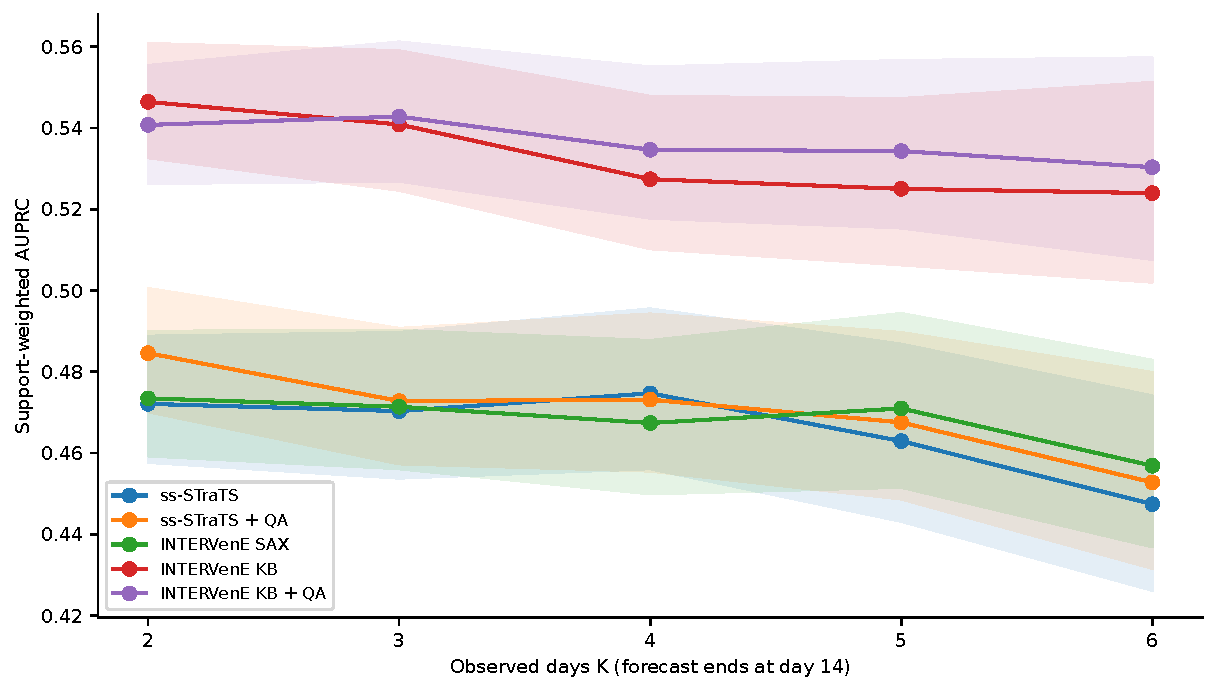
\includegraphics[width=.9\textwidth]{updated_window_sensitivity}
\caption{Weighted AUPRC for predictions made from day two to day six, with follow-up through day 14. Model weights were fixed across cutoffs. Shading indicates 95\% intervals.}
\label{fig:windows}
\end{figure}

\subsection{Transfer to held-out hospitals}
KB retained discrimination at all six hospitals when each was held out from training (Table~\ref{tab:loo}). Weighted AUPRC ranged from 0.431 to 0.539 across hospitals and weighted AUROC from 0.725 to 0.828. The corresponding pooled estimates, 0.527 and 0.803, lay within these ranges, although some hospitals had lower scores. Each hospital contributed a different patient population, so these comparisons cannot quantify the loss attributable to moving a model to a new site.

\begin{table}[htbp]
\centering\small
\caption{KB performance when the evaluated hospital is excluded from fitting.}
\label{tab:loo}
\resizebox{\textwidth}{!}{\begin{tabular}{lrrrr}
\toprule
Held-out hospital & Admissions & PR reference & AUPRC (95\% CI) & AUROC (95\% CI) \\
\midrule
Barzilai University Medical Center & 5,978 & 0.236 & 0.516 [0.500, 0.534] & 0.788 [0.779, 0.797] \\
Bnai Zion Medical Center & 3,253 & 0.266 & 0.539 [0.520, 0.563] & 0.776 [0.765, 0.788] \\
Galilee Medical Center & 5,899 & 0.158 & 0.481 [0.462, 0.501] & 0.829 [0.820, 0.837] \\
Hillel Yaffe Medical Center & 5,063 & 0.228 & 0.464 [0.449, 0.481] & 0.771 [0.762, 0.780] \\
Tzafon Medical Center (Poria) & 2,388 & 0.251 & 0.431 [0.409, 0.457] & 0.725 [0.710, 0.740] \\
Shamir Medical Center & 7,348 & 0.264 & 0.514 [0.499, 0.530] & 0.770 [0.762, 0.779] \\
\bottomrule
\end{tabular}
}
\par\smallskip\parbox{\textwidth}{\footnotesize The precision--recall reference is the mean outcome prevalence at each hospital, weighted by positive counts ($\sum_j p_j^2/\sum_j p_j$). Supplementary Table~S3 gives the individual prevalences. At Bnai Zion, only 1,710 of 2,000 bootstrap draws were valid, below the prespecified threshold for reliable intervals. All other aggregate intervals had 2,000 valid draws.}
\end{table}
\noindent\textit{Author note: Confirm with coauthors whether hospitals may be identified by name; anonymize consistently if required.}

At every held-out hospital, AUPRC exceeded the reference calculated from that hospital's outcome prevalences. The six KB fits alone took more than a week, which made repeating the analysis for all baseline models impractical. The comparison with other models therefore comes from the pooled test set. Supplementary Table~S7 breaks down pooled-model performance by age, sex, and hospital. Infection occurred in only two test admissions among patients younger than 55 and in none of the 495 test admissions at Bnai Zion, where aggregate discrimination across all eight outcomes was consequently undefined. Supplementary Table~S8 reports calibration.

\subsection{Embedding structure}
At a fixed timestamp, the closest embeddings were the START and END of the same concept (median cosine distance 0.180). Distances increased from pairs sharing an abstraction (0.226) to those sharing only an underlying variable (0.443) and those with different underlying variables (0.590). Figure~\ref{fig:embedding} shows this organization for the whole vocabulary and in more detail for glucose. The trained embeddings preserved the relationship between a concept's boundaries and its place in the clinical hierarchy. Whether an END token attends to the START of its own interval is a separate question that embedding distances cannot answer.
\begin{figure}[p]
\centering
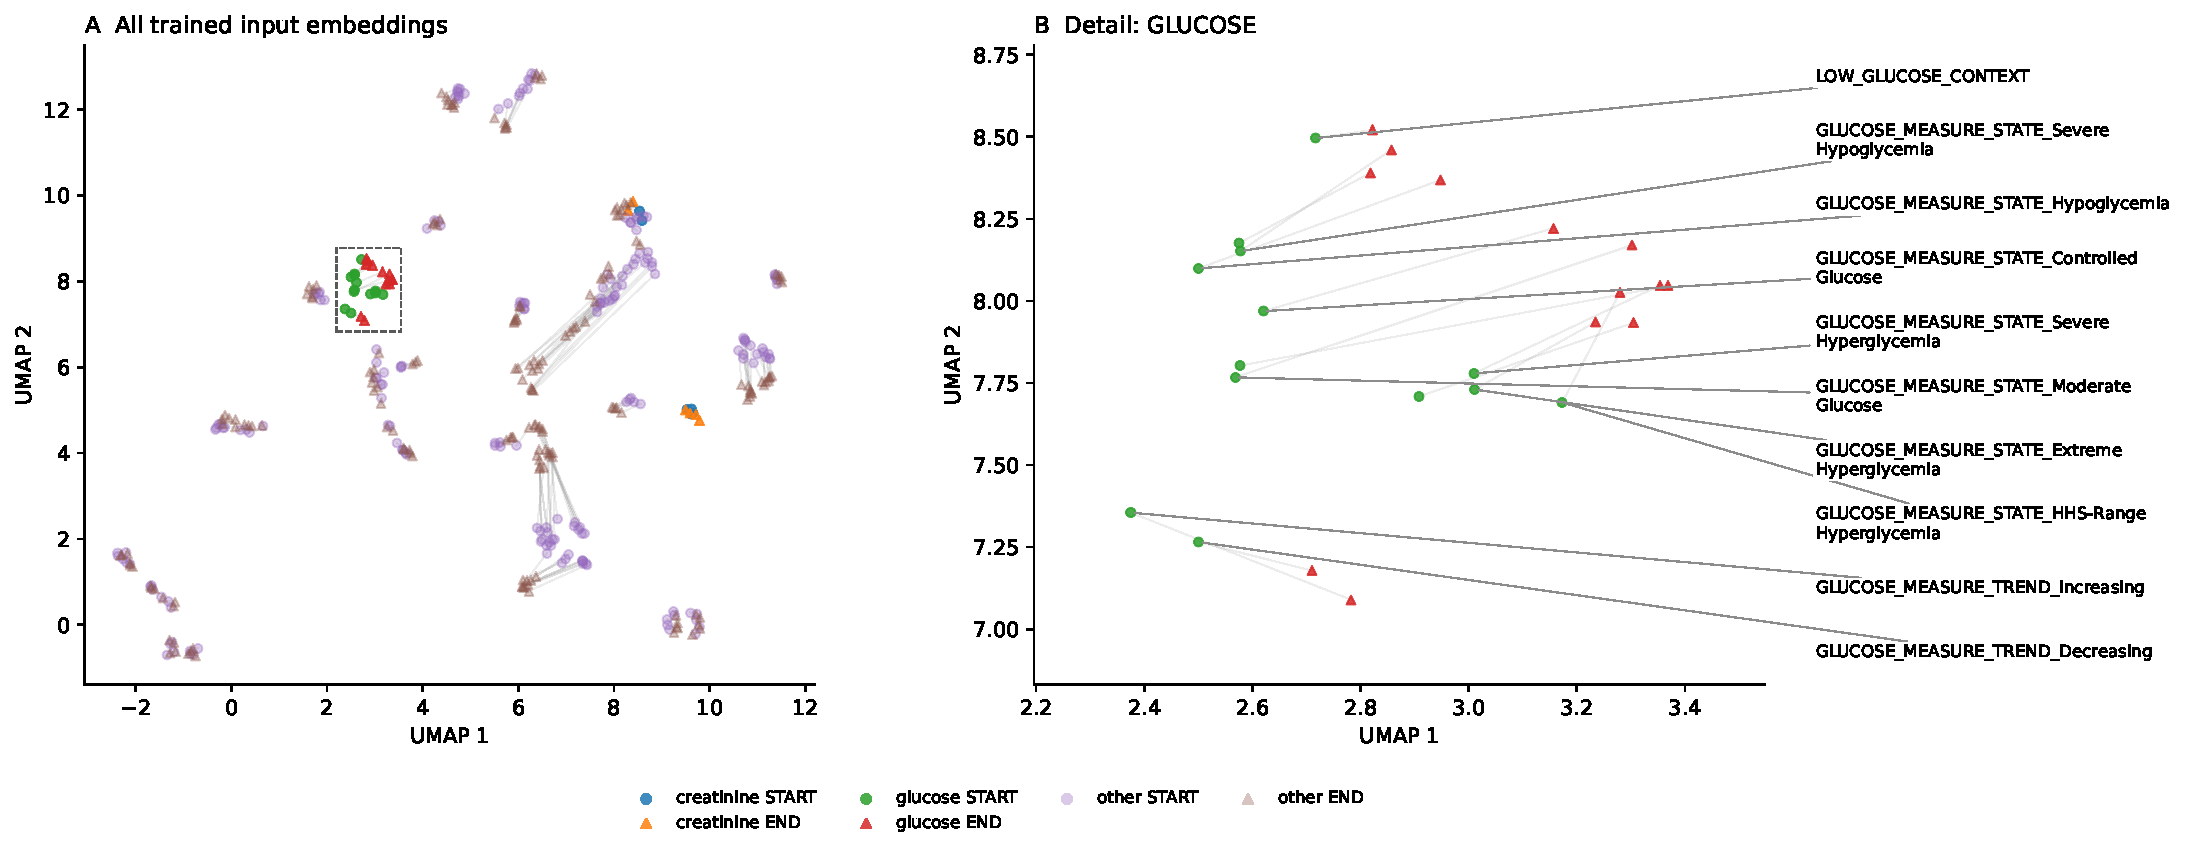
\includegraphics[width=.65\textwidth,trim=0 45 610 0,clip]{updated_embedding_umap}\\[8pt]
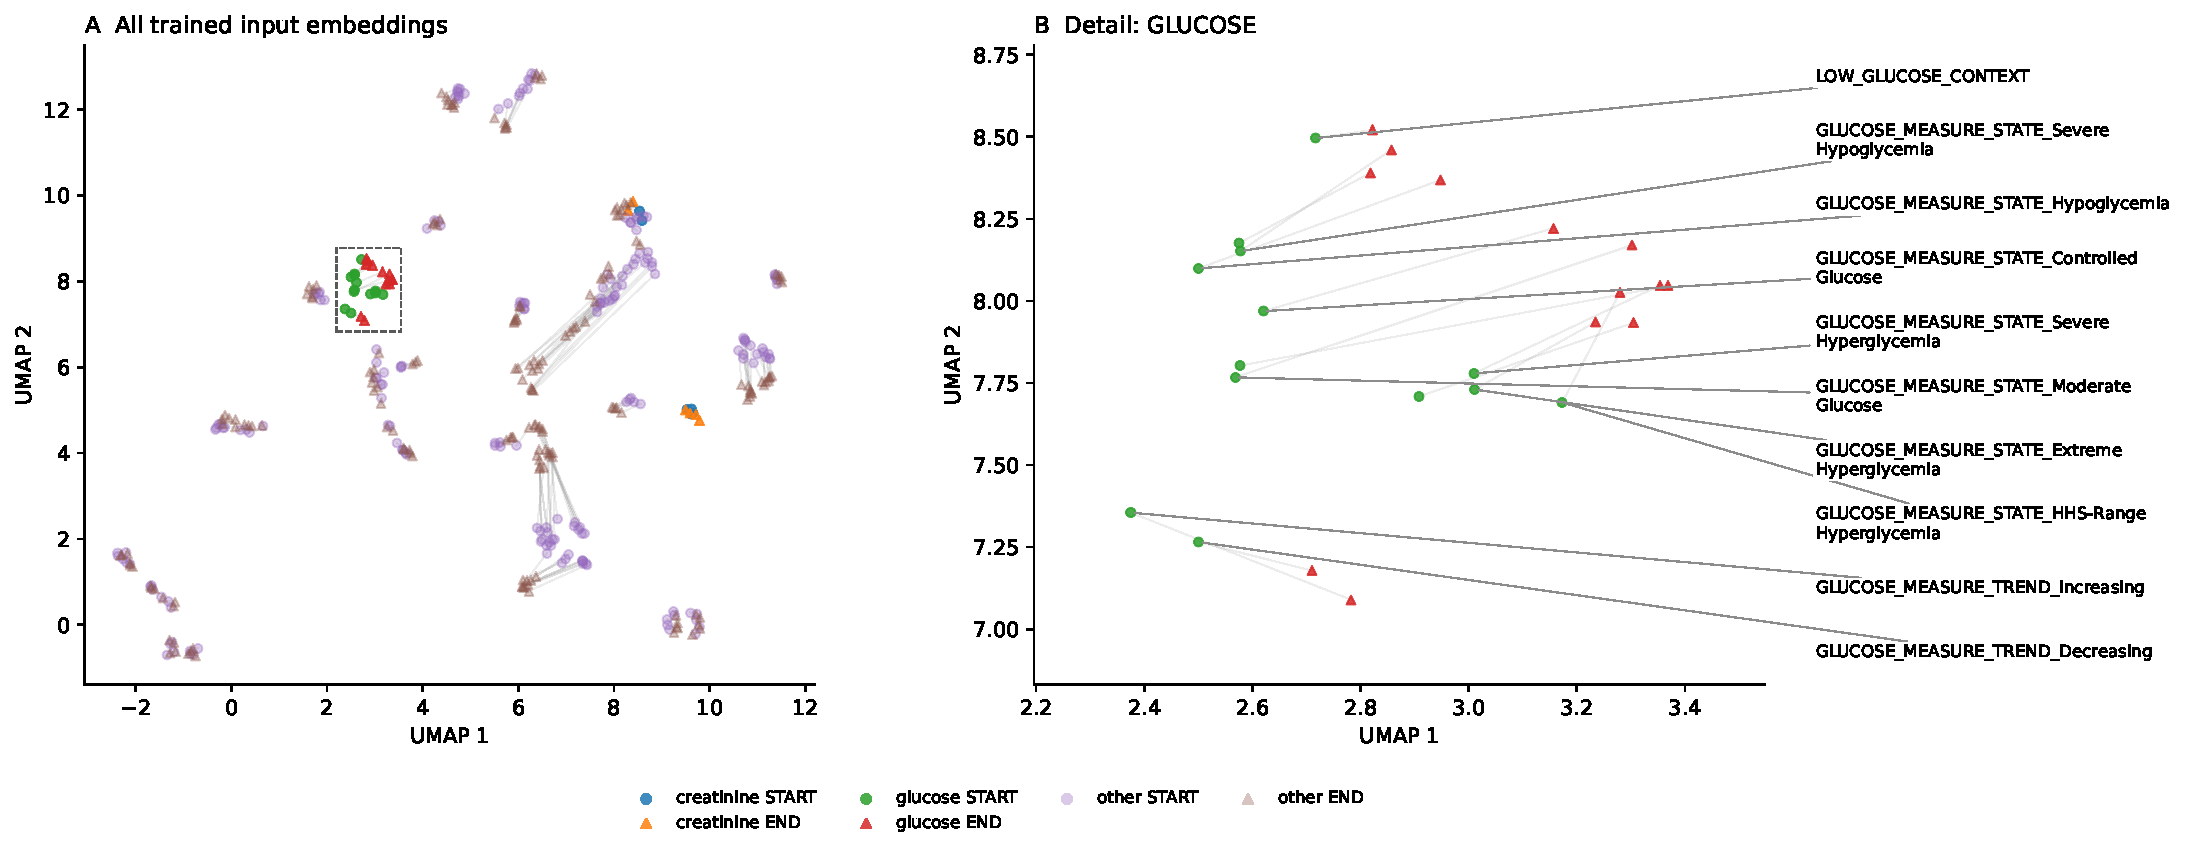
\includegraphics[width=\textwidth,trim=480 45 0 0,clip]{updated_embedding_umap}
\caption{Trained input embeddings at a fixed timestamp. The upper panel shows the UMAP projection of the vocabulary. The lower panel enlarges the glucose family in the same projection. Circles denote START tokens and triangles denote END tokens. The encoder incorporates the clinical hierarchy, and the reported cosine distances were calculated in the original embedding space.}
\label{fig:embedding}
\end{figure}

\subsection{Named-concept attribution and the previous clinical findings}
In KB+QA, the clinical token at a given position identifies a state, trend, event, context, or guideline assessment. Summing transcoder contributions at positions with the same name lets us report a contribution from \emph{decreasing glucose}, for example, even when that trend spans several readings. The vocabulary supplies the name, and the transcoder estimates the model's sensitivity at each occurrence. Clinical states accounted for many of the largest contributions. Every outcome had a QA pattern among its top 30 concepts, although the highest-ranked QA pattern ranged from seventh to twenty-fourth across outcomes.

A falling glucose trend contributed toward higher predicted hypoglycemia risk. When the insulin-after-hyperglycemia pattern was scored false, it contributed toward lower predicted risk and ranked seventh for both hypoglycemia outcomes. In the clinical study, greater adherence to this recommendation was associated, after propensity weighting, with higher odds of hypoglycemia (OR 1.283, 95\% CI 1.163--1.416) and lower odds of severe hyperglycemia (OR 0.220, 0.202--0.239) \citep{oded2027kineret-jbi}. The direction of the attribution is consistent with this trade-off. A pattern scored false leaves open how much insulin the patient received and why care differed from the recommendation.

Routine glucose monitoring was the highest-ranked QA concept for mortality and contributed toward lower predicted risk. The clinical study also found lower odds of 30-day mortality with greater adherence to routine monitoring after propensity weighting (OR 0.870, 95\% CI 0.809--0.937) \citep{oded2027kineret-jbi}. That analysis accounted for measured confounders, although residual confounding was possible. The attribution describes a predictive association and cannot establish that monitoring prevented deaths. Despite the direction of this particular contribution, adding all QA inputs reduced the model's ability to distinguish admissions ending in a death marker from those without one during the forecast period.

For all 300 admissions, attaching the transcoders left the original risk predictions unchanged (maximum absolute difference in risk logits, 0). Reconstruction was less complete. Across the four layers, the transcoders explained only part of the variance in held-out layer outputs ($R^2=0.396$--$0.514$). The encoder continued to use its original layer outputs for prediction. The unexplained variance therefore limits the feature-based explanation, even though the predictions themselves were unchanged. Agreement with selected findings from the clinical study lends these exploratory explanations clinical plausibility. Supplementary Table~S9 gives reconstruction and sparsity by layer. Table~S10 lists the highest-ranked QA concepts.

\subsection{Stability of the clinical abstractions}
For the 500 people in the perturbation analysis, the Mediator assigned the same state label to 97.6\% of covered time and the same trend label to 98.0\% after we added noise of 5\% of local threshold spacing. When we removed 10\% of observations, agreement was 97.4\% for states and 95.3\% for trends. The corresponding losses of baseline coverage were 2.0\% and 3.2\%. These estimates describe the stability of numeric states and trends under modest changes in the measurements. QA patterns and downstream predictions were outside this analysis. Supplementary Table~S11 reports intervals and coverage for each perturbation.
